\documentclass{article}

\usepackage[utf8]{inputenc}
\usepackage[T1]{fontenc}

\usepackage{tikz-er2}
\usetikzlibrary{positioning}
\usetikzlibrary{shadows}

\usepackage{subcaption}
\usepackage{enumitem}
\usepackage{hyperref}



\begin{document}
\title{Chess Openings Database Specification}
\author{Yoan Geran \and Colin Geniet}
\maketitle

\tableofcontents

\section{Logical design}
\subsection{Entity relationship}
As a reminder, the EER schema from the first part is in figure \ref{eer}.
The translated database schema is in figure \ref{db}.


\tikzstyle{every entity} = [top color=white, bottom color=blue!30, 
                            draw=blue!50!black!100, drop shadow]
\tikzstyle{every weak entity} = [drop shadow={shadow xshift=.7ex, 
                                 shadow yshift=-.7ex}]
\tikzstyle{every attribute} = [top color=white, bottom color=yellow!20, 
                               draw=yellow, node distance=1cm, drop shadow]
\tikzstyle{every relationship} = [top color=white, bottom color=red!20, 
                                  draw=red!50!black!100, drop shadow]

\begin{figure}
\caption{EER schema}
\label{eer}
\begin{center}
\scalebox{.80}{
\begin{tikzpicture}[every edge/.style={link}]
    \node[entity] (game) {Game};
    
    \node[relationship] (white) [below right= 0cm and 1cm of game] {white} edge node [auto] {1} (game);
    \node[relationship] (black) [above right= 0cm and 1cm of game] {black} edge node [auto,swap] {1} (game);
    \node[entity] (player) [above right= 0cm and 1cm of white] {Player} edge (white);
    \draw[link] (player) edge (black);
    
    \node[relationship] (gevent) [above left= 1cm and 0cm of game] {in event} edge node [auto] {1} (game);
    \node[entity] (event) [left= 0.5cm of gevent] {Event} edge (gevent);
    
    \node[relationship] (gopening) [left= 5cm of game] {played in} edge (game);
    \node[entity] (opening) [above= 1cm of gopening] {Opening} edge (gopening);
    \node[relationship] (variation) [above= 0.5cm of opening] {variation};
    \draw[link] (opening.70) edge (variation.283);
    \draw[link] (opening.110) edge (variation.257);
    
    \node[draw,circle,top color=white, bottom color=green!20, draw=green!50!black!100, drop shadow] (obj_is) 
         [above= 6cm of game] {D} edge (game) edge (opening) edge (event) edge (player);
    \node[entity] (object) [above= 1cm of obj_is] {Object} edge node {$\bigcup$} (obj_is);
    
    \node[relationship] (owns) [left= of object] {owns} edge [total] node [auto] {1} (object);
    \node[entity] (user) [left= of owns] {User} edge (owns);
    \node[relationship] (edit) [below left= 1cm and 1.2cm of object] {can edit} edge [total] (object) edge (user);
    
    \node[relationship] (on) [above= 1cm of object] {on} edge (object);
    \node[entity] (comment) [left= of on] {Comment} edge [total] node [auto] {1} (on);
    \node[relationship] (from) [above= 0.8cm of user] {from} edge (user) edge [total] node [auto] {1} (comment);
\end{tikzpicture}
}
\end{center}
\end{figure}

\begin{figure}
\caption{Relational schema}
\label{db}
\begin{center}
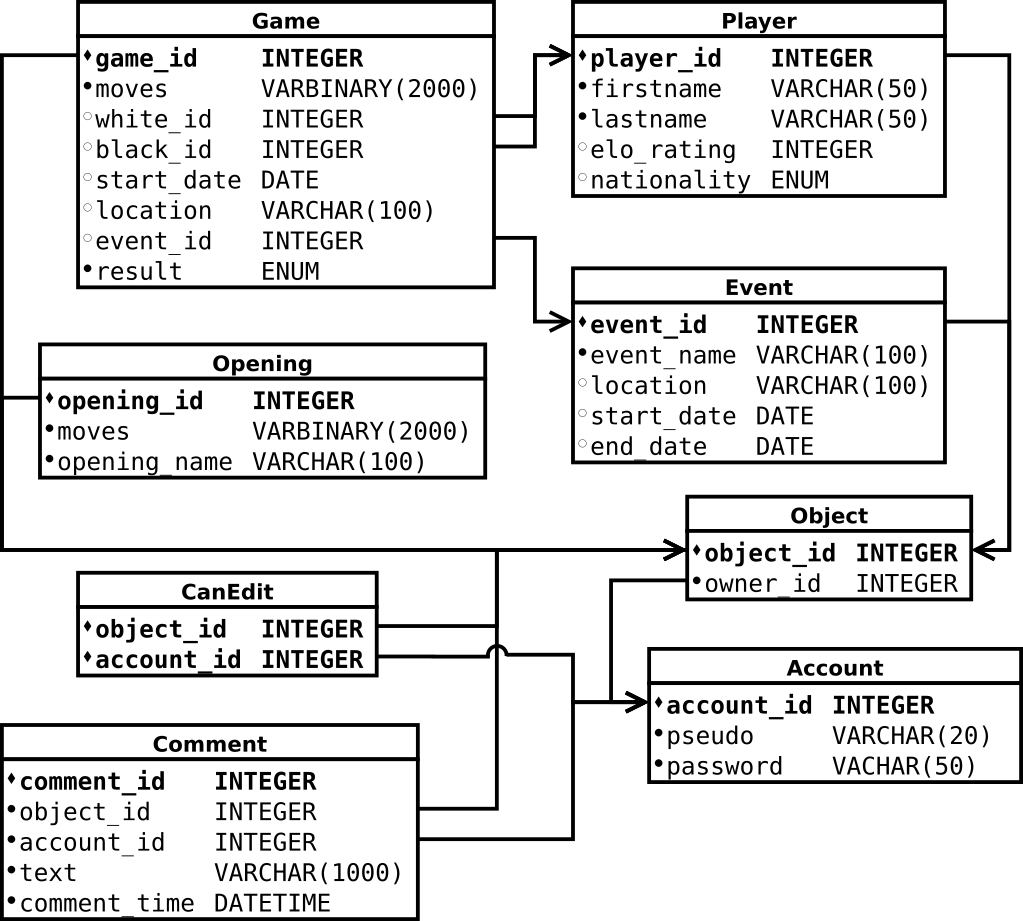
\includegraphics[scale=0.6]{relational}
\end{center}
Bold denotes primary keys, black and white dots denotes required and optional attributes respectively.
\end{figure}


\subsection{Relational schema}
\begin{verbatim}

\end{verbatim}

\subsection{Integrity Constraints}
\begin{itemize}
\item \verb|moves| attributes in entities \verb|Game| and \verb|Opening| must represent
valid sequences of chess moves starting from the initial chess position.

\item Relationships \verb|opening| and \verb|variation| must respect the values of \verb|moves|
attributes in respective entities.
Precisely, opening $A$ is a variation on opening $B$ if and only if the move sequence
of $A$ starts (in the prefix meaning) with the move sequence of $B$.
Similarly, game $A$ has $B$ as an opening if and only if the move sequence of $A$ starts
with the move sequence of $B$.

\item An user can edit any object they owns.
\end{itemize}



\section{Design choices}

\subsection{Relationship cardinalities}
While some cardinality constraints on relationships may seem too weak,
they are justified by special cases. For instance :
\begin{itemize}
\item \verb|white| and \verb|black| relationships need not to be total with regard to the game, as players may be unknown.

\item \verb|opening| relationship is neither total nor limited with regard to the game,
as a game may match several openings (an opening and its variation), or none if played with unconventional opening.
\end{itemize}

\subsection{The \texttt{Object} entity}
The \verb|Object| entity regroups all objects that can be manipulated (i.e.\ created, modified, commented \dots) by users,
that is games, openings, events, \dots
Its use abstracts manipulation operations, when they are independent from the precise entity.

For instance, a comment on an object is not affected in any way by the exact type this object.
Thus, comments are linked to \verb|Object| entities, and not directly to a \verb|Game| etc.
Similarly, the ownership notion is independent from the object.

\subsection{Chess moves representation}
Obviously, chess moves will be a very important --- and big --- part of this database.
Thus, finding an efficient representation for them is important.
The one we settled for is to represent any of the 64 squares by a byte.
A move is represented by two bytes, and a sequence of moves by a bytes sequence.

While not human readable, this representation is quite compact, totally unambiguous,
has an unique representation for any given move, and uses has constant representation
size for a move.

All this advantages are important when searching in the database for games starting
with a given move sequence, as the search is simply a prefix lookup.

The other representation we considered are :
\begin{itemize}
\item Algebraic notation is the most standard, but has problems with ambiguity
(two valid strings can represent the same move), making search much more complicated.
Additionally, it uses more space, and it has non-constant representation size.

\item Representing the start and end squares in plain text mostly keeps the advantages
of our representation while being human readable. However, it do uses twice more space.
Since having a human readable internal representation is not very useful,
we ruled it out.
\end{itemize}


\paragraph{Detailed representation}
Chess board squares are numbered from left to right, and from bottom to top,
starting with 0. Thus, \verb|a1| is numbered as 0, \verb|a8| as 7, \verb|b1| as 8, \dots
The square number is directly encoded in the six lower end bits of a byte, which is considered as a character.

For promotions, the two remaining higher end bits of the end square are used to represent the piece promoted to,
encoded as Queen=0 (values in range 0--63), Knight=1 (64--127), Rook=2 (128--191), Bishop=3 (192--255).
For instance, a pawn promoting on column \verb|a| will be represented as 6--7 for a queen promotion,
6--71 for a Knight promotion, 6--135 for a Rook promotion.

Note that castling is represented by the King move.


\section{Functional Analysis}
\subsection{Search}
Any user can search the database to obtain a list of games matching some criteria.
Criteria are :
\begin{itemize}[noitemsep]
\item A sequence of moves that must match the beginning of the game.
\item Games using a given opening (used instead of a sequence of moves).
\item The players names/nationality. This criteria can be set for any side
(e.g.\ one player is R.J.Fischer) or a specific one (e.g.\ black is R.J.Fischer)
\item Game date (e.g. played after Jan. 20, 2001)
\item Event
\item Location
\end{itemize}

In addition to the list of games, the search results includes the followings :
\begin{itemize}[noitemsep]
\item Number of matching games.
\item Win frequency for each player, and draw frequency.
\item Openings matching the initial sequence of moves.
When using an opening as search criteria, this means less specific openings.
\item Most used move and opening (after the initial sequence of moves/opening, if any).
\end{itemize}

Users can select games, openings, players or events to view details.
\begin{itemize}
\item For games, the game moves can be viewed, as well as result, players, date, location, event,
and matching opening(s).
\item For openings, the opening moves can be viewed, as well as more generic openings, variations, name
and games using this opening.
\item For players, the name, nationality and Elo rating and list of games can be viewed.
\item For events, the name, location, date and list of games can be viewed.
\end{itemize}

Obviously, lists are not fully displayed if too big.
They are sorted by :
\begin{itemize}[noitemsep]
\item Number of matching games for openings.
\item Players Elo rating for games.
\item Elo rating for players.
\item Date (most recent) for events.
\end{itemize}


\subsection{Database modification}
An user can create an account, which creates a corresponding \verb|User| entity.
A registered user can then add new games, players, openings and events to the database.
\begin{itemize}
\item Games can be added manually, or imported from a \verb|pgn| file.
\item Openings may be created from scratch, or as variations on an existing opening.
\end{itemize}

An users owns any object they created, and has edit rights on objects they own.
Users can modify or delete any object they have edit rights on.

Any registered user can post comments on any object.


\end{document}